\documentclass{rapport}
\usepackage[utf8]{inputenc}

\usepackage{pifont} % Pour les symboles appelés par la macro \ding
\usepackage{url} % Comme son nom l'indique, pour les url...

\usetikzlibrary{positioning} % Bibliothèque tikz pour positionner des nœuds relativement à d'autres

\usepackage[colorlinks, citecolor=red!60!green, linkcolor=blue!60!green, urlcolor=magenta]{hyperref} % Pour que les liens soient cliquables. Les options permettent de mettre les liens en couleur.

\usepackage{algorithm}
\usepackage{algo}
\usepackage{colorationSyntaxique}


% Pour un rapport en français 
% \usepackage[francais]{babel} % Commenter pour un rapport en anglais
% \renewcommand\bibsection{\section*{Bibliographie}} % Commenter pour un rapport en anglais

\englishTitlePage % Décommenter pour une page de titre en anglais


\pagestyle{fancy}
\renewcommand{\sectionmark}[1]{\markboth{\thesection.\ #1}{}}
\fancyfoot{}

\fancyhead[LE]{\textsl{\leftmark}}
\fancyhead[RE, LO]{\textbf{\thepage}}
\fancyhead[RO]{\textsl{\rightmark}}

\def\Latex{\LaTeX\xspace}
\def\etc{\textit{etc.}\xspace}



\title{Hardware Performance Counters}
\author{Francois Flandin}
\supervisor{Sid Touati}
\date{Second semestre de l'année 2024-2025}

\universityname{Université Côte d'Azur} % Nom de l'université.
\type{TER} % Type de document
\formation{Master Informatique} % Nom de la formation

% Retrouver les autres options possibles dans le document rapport.pdf

\begin{document}

  \maketitle

  \begin{abstract}
    Calmos le ramoloss, l'abstract c'est pas pour tout de suite
  \end{abstract}

  \clearpage
  \tableofcontents
  \clearpage
  \section{Introduction}
  If you wish to explore the details of the work done for the project, the project's code is hosted on GitHub at https://github.com/omelette-bio/projet-tutorat-s2-m1

  \clearpage
    
  \section{Hardware Performance Monitoring on AMD CPUs}

  \begin{figure}[H]
        \centering
        \makebox[\textwidth]{
    	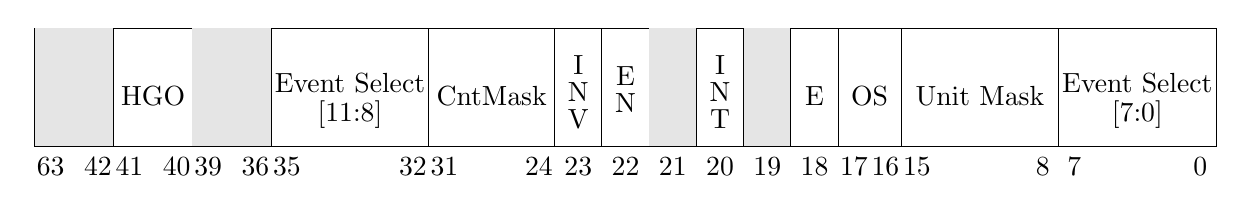
\begin{tikzpicture}
    		% Draw the main box
    		\draw (0,0) rectangle (15,1.5);
    
    		% Draw sub-boxes
    		\draw (0,0) -- (0,1.5); % debut zone reservee
    
    		\node[anchor=south] at (0.2,-0.5) {63};
    		\fill[gray!20] (0,0) rectangle (1,1.5);
    		\node[anchor=south] at (0.8,-0.5) {42};
    
    		\draw (1,0) -- (1,1.5);
        
            \node[anchor=south] at (1.2,-0.5)	{41};
    		\node[anchor=south] at (1.5,0.4)	{HGO};    		
    		\node[anchor=south] at (1.8,-0.5)	{40};
        
            \draw (2,0) -- (2,1.5);
            
            \node[anchor=south] at (2.2,-0.5)	{39};
            \fill[gray!20] (2,0) rectangle (3,1.5);
            \node[anchor=south] at (2.8,-0.5)	{36};
            
            \draw (3,0) -- (3,1.5);
    
            \node[anchor=south] at (3.2,-0.5)	{35};
    		\node[anchor=south] at (4,0.1)	{\shortstack{Event Select\\{[11:8]}}};
    		\node[anchor=south] at (4.8,-0.5)	{32};
    
            \draw (5,0) -- (5,1.5);
            
            \node[anchor=south] at (5.2,-0.5)	{31};
    		\node[anchor=south] at (5.8,0.4)	{CntMask};
    		\node[anchor=south] at (6.4,-0.5)	{24};
      
            \draw (6.6,0) -- (6.6,1.5);
    
    		\node[anchor=south] at (6.9,-0.5) {23};
    		\node[anchor=south] at (6.9,0.1)  {\shortstack{I\\N\\V}};
    
    		\draw (7.2,0) -- (7.2,1.5);
    
    		\node[anchor=south] at (7.5,-0.5) {22};
    		\node[anchor=south] at (7.5,0.3)  {\shortstack{E\\N}};
    
    		\draw (7.8,0) -- (7.8,1.5);
    
    		\node[anchor=south] at (8.1,-0.5) {21};
    		\fill[gray!20] (7.8,0) rectangle (8.4,1.5);
    
    		\draw (8.4,0) -- (8.4,1.5);
    
            \node[anchor=south] at (8.7,-0.5)	{20};
    		\node[anchor=south] at (8.7,0.1)  {\shortstack{I\\N\\T}};
    
    		\draw (9,0) -- (9,1.5);
    
    		\node[anchor=south] at (9.3,-0.5)	{19};
    		\fill[gray!20] (9,0) rectangle (9.6,1.5);
    
    		\draw (9.6,0) -- (9.6,1.5);
    
    		\node[anchor=south] at (9.9,-0.5) {18};
    		\node[anchor=south] at (9.9,0.4)  {E};
    
    		\draw (10.2,0) -- (10.2,1.5);
    
    		\node[anchor=south] at (10.4,-0.5)	{17};
    		\node[anchor=south] at (10.6,0.4)	{OS};    		
    		\node[anchor=south] at (10.8,-0.5)	{16};
    
    		\draw (11,0) -- (11,1.5);
    
    		\node[anchor=south] at (11.2,-0.5)	{15};
    		\node[anchor=south] at (12,0.4)  {Unit Mask};
    		\node[anchor=south] at (12.8,-0.5)  {8};
    
    		\draw (13,0) -- (13,1.5);
    
    		\node[anchor=south] at (13.2,-0.5)  {7};
    		\node[anchor=south] at (14,0.1)	{\shortstack{Event Select\\{[7:0]}}};
    		\node[anchor=south] at (14.8,-0.5)	{0};
    	\end{tikzpicture}
	   }
	   \label{fig:figure1}
	   \caption{AMD Bit Repartition of \texttt{Event Select MSRC001\_020[A,8,6,4,2,0]}}
	\end{figure}

  \section{Hardware Performance Monitoring on INTEL CPUs}
  \pageblanche
  \bibliographystyle{apalike-fr}
  \bibliography{biblio}

\end{document}
